%! Author = Leonardo Cruciani
%! Date = 29/03/2025

% Preamble
\documentclass[11pt]{article}

% Packages
\usepackage[top=1in, bottom=1.2in, left=1in, right=1in]{geometry}
\usepackage{amsmath}
\usepackage{upgreek}
\usepackage{graphicx}
\usepackage{wrapfig}
\usepackage{hyperref}
\usepackage{tikzexternal}
\usepackage{amsfonts}
\setlength{\parindent}{0pt}
\newcommand{\atan}{\,\text{atan}}
\newcommand{\sgn}{\,\text{sgn}}
\newcommand{\pdf}{\,\text{pdf}}

\author{Leonardo Cruciani}
\title{Forecasting VaR using Garch and KDE}
% Document
\begin{document}
    \maketitle
    \section{Introduction}
        This work aims to describe the usage of Kernel Density Estimation methods in the context of Value at Risk (VaR) forecasting.
        It mainly consists of 2 parts:
        \begin{itemize}
            \item In section~\ref{sec:replication}, I use KDE to help solve a numerically intensive problem in the replication of paper~\cite{thorsten}.
            In particular, the paper uses a Truncated Skewed Lèvy (TSL) distribution to model the standardized returns (where the volatilities are estimated via GARCH),
            making the forecasted VaR proportional to Truncated Skewed Lèvy percentiles.
            Because the TSL distribution is defined in terms of its characteristic function (does not have a close form solution) and depends on several parameters, making the estimation of the parameters difficult, the KDE is then used to obtain a faster estimate.
            \item In section~\ref{sec:direct}, I get rid of the TSL distribution hypothesis and instead use directly the kernel density estimated distribution to calculate the percentiles for VaR forecasting.
        \end{itemize}
        As the Garch volatility estimation is common to both parts, I start by describing it in section~\ref{sec:garch}.
        I conclude by comparing the results of the two methods in section~\ref{sec:comparison}.

    \section{Data}
        The dataset contains the closing prices of some popular indices (S\&P500, FTSE, Eurostoxx50 and Euronext100) from 2006 to 2024.
        The dataset is split in two, with the first 11 years being used for training and the last 7 years for testing.
        From the dataset the log returns are computed, expressed in percentage terms, and aggregated for 5, 10 and 20 days.

    \section{Garch} \label{sec:garch}
        Since its inception, various Garch models have been used in the field of finance.
        In the paper~\cite{thorsten} an augmented Garch model that nests all the most commonly used (e.g. Garch(1,1), GJR-Garch, Aparch, etc) is proposed.
        In this work I will resort to a simpler Power Garch model with leverage effect to model the volatility $\sigma_t$:
        \begin{equation}
            \sigma_t^\kappa = \omega
            + \alpha \left|\epsilon_{t-1}\right|^\kappa
            + \beta \sigma_{t-1}^\kappa
            + \gamma \left|\epsilon_{t-1}\right|^\kappa I_{[\epsilon_{t-1}<0]}
        \end{equation}
        Where $\epsilon_t \sim D(0,1)$ are independent shocks distributed according to a \textit{standardized distribution} $D(0,1)$.
        In the paper~\cite{thorsten} and in section~\ref{sec:replication} this $D(0,1)$ distribution is the TSL calibrated on historical data, while in section \ref{sec:direct} the KDE distribution is used.
        The parameters to be estimated are: $\alpha$, which models the sensitivity of the volatility to the shock; $\beta$, which models the persistence of the volatility; $\gamma$, which models the leverage effect; the exponent $\kappa$ (typically $\simeq 2$) and the so called (when $\kappa=2$) long term variance $\omega$.\\
        To model the return $r_t$ I used the following model:
        \begin{equation}
                r_t = \mu + \sigma_t \epsilon_t,
        \end{equation}
        Where the mean $\mu$ can be safely assumed to be constant for medium to short term returns.
        The parameters of the Garch are calibrated on historical data and the model is then used to forecast the next period variance $\hat \sigma_{t+1}^2$ as returns become available.
        Therefore, the closing prices in the dataset are standardized following the formula:
        \begin{equation}
            z_t = \frac{r_t - \hat \mu}{\hat \sigma_t}
        \end{equation}
        where $\hat \mu$ and $\hat \sigma$ are obtained from the Garch.
        \begin{center}
\begin{tabular}{lclc}
\toprule
\textbf{Dep. Variable:} &            Returns             & \textbf{  R-squared:         } &     0.000   \\
\textbf{Mean Model:}    &         Constant Mean          & \textbf{  Adj. R-squared:    } &     0.000   \\
\textbf{Vol Model:}     & Asym. Power GARCH (power: 1.8) & \textbf{  Log-Likelihood:    } &   -3683.10  \\
\textbf{Distribution:}  &             Normal             & \textbf{  AIC:               } &    7376.21  \\
\textbf{Method:}        &       Maximum Likelihood       & \textbf{  BIC:               } &    7405.84  \\
\textbf{}               &                                & \textbf{  No. Observations:  } &    2769     \\
\textbf{Date:}          &        Tue, Apr 08 2025        & \textbf{  Df Residuals:      } &    2768     \\
\textbf{Time:}          &            17:06:58            & \textbf{  Df Model:          } &     1       \\
\bottomrule
\end{tabular}
\begin{tabular}{lccccc}
            & \textbf{coef} & \textbf{std err} & \textbf{t} & \textbf{P$> |$t$|$} & \textbf{95.0\% Conf. Int.}  \\
\midrule
\textbf{mu} &       0.0263  &    1.466e-02     &     1.792  &      7.309e-02       &   [-2.458e-03,5.501e-02]    \\
                  & \textbf{coef} & \textbf{std err} & \textbf{t} & \textbf{P$> |$t$|$} & \textbf{95.0\% Conf. Int.}  \\
\midrule
\textbf{omega}    &       0.0247  &    5.356e-03     &     4.605  &      4.124e-06       &   [1.417e-02,3.516e-02]     \\
\textbf{alpha[1]} &     0.0000    &    2.057e-02     &   0.000    &          1.000       &   [-4.032e-02,4.032e-02]    \\
\textbf{gamma[1]} &       0.2059  &    3.003e-02     &     6.858  &      7.000e-12       &     [  0.147,  0.265]       \\
\textbf{beta[1]}  &       0.8818  &    1.835e-02     &    48.043  &        0.000         &     [  0.846,  0.918]       \\
\bottomrule
\end{tabular}
\caption{Constant Mean - Asym. Power GARCH (power: 1.8) Model Results}
\end{center}

Covariance estimator: robust

    \section{Paper Replication} \label{sec:replication}
        \subsubsection{Truncated Skewed Levy}
        The $TSL(\mu, c, \alpha, \lambda, \beta)$ is defined through  its characteristic function $\varphi_{TSL}(k) = \exp\big(-\psi(k; \mu, c, \alpha, \lambda, \beta)\big)$ where:
        \begin{equation}
            \begin{aligned}
                \psi(k; \mu, c, \alpha, \lambda, \beta) &= ik\mu \,+\\
                                                    & + c^{\alpha}\left[\frac{\lambda^2-(k^2+\lambda^2)^{\alpha/2}}{\cos(\pi \alpha/2)}\cos\left(\alpha \atan \left(\frac{|k|}{\lambda}\right)\right)\right] \times \\
                                                    & \times \left[ 1+ i \sgn(k) \beta \tan \left(\alpha\left(\frac{|k|}{\lambda}\right)\right) \right]
            \end{aligned}\label{eq:char_func}
        \end{equation}
        for all $k \in \mathbb{R}$.
        The parameters have the following meaning (see figure~\ref{fig:parameters}):
        \begin{itemize}
            \item $\mu$ is the location parameter.
            \item $c >0$ is the scale parameter.
            \item $\alpha \in (0,2] \setminus\{1\} $ is the characteristic exponent, which defines the overall shape of the PDF, and especially the fatness of the tails. To give an intuition, the closer $\alpha$ is to $2$, the closer the $TSL$ approximates a Gaussian.
            \item $\lambda > 0$ is the cutoff parameter, which is responsible for making the moments of the TSL well-defined.
            \item $\beta \in [-1, 1]$ is the skewness parameter: the PDF of the TSL is skewed to the right for negative $\beta$ and to the left for positive $\beta$.
        \end{itemize}
        The PDF of the distribution can be obtained by fourier transforming the characteristic function:
        \begin{equation}
            \pdf_{TSL}(x; \mu, c, \alpha, \lambda, \beta) =  \frac{1}{2\pi}\int_{\mathbb R} \exp\big(-ikx-\psi(k; \mu, c, \alpha, \lambda, \beta)\big)\,dk\label{eq:pdf}
        \end{equation}
        \begin{figure}[h!]
            \label{fig:parameters}
            \centering
            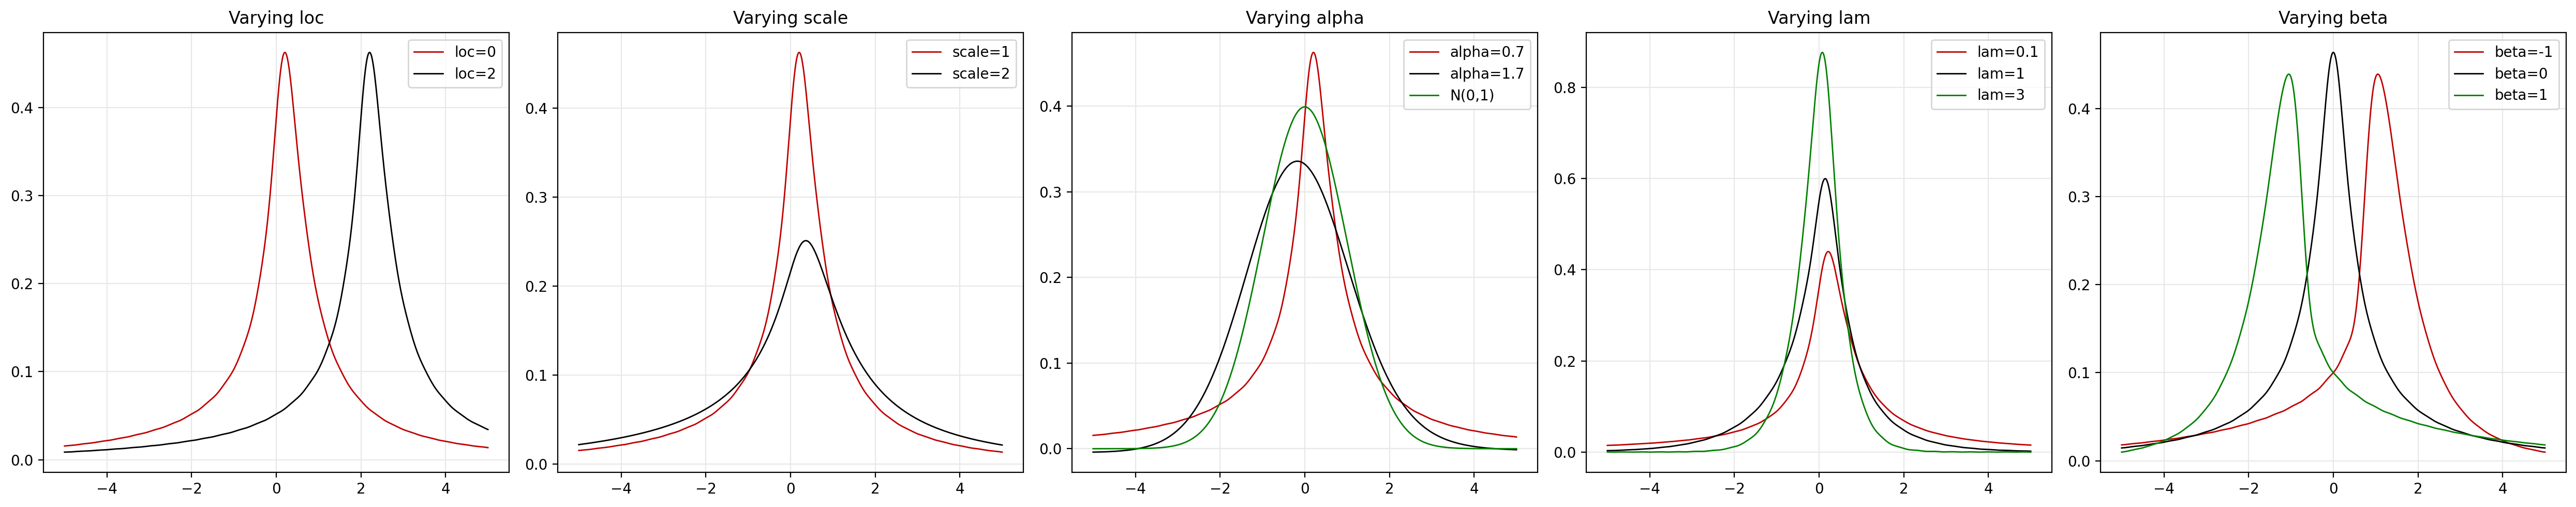
\includegraphics[width=0.9 \linewidth]{parameters}
            \caption{TSL PDF. Baseline parameters: $\mu=0, \,c=1,\, \alpha = 0.7, \, \lambda = 0.2,\, \beta =-0.2$}
        \end{figure}
        The fundamental property of this distribution which makes it well suited for the task of estimating longer horizon variances is its convolution property.
        In particular the PDF satisfies:
        \begin{equation}
            \pdf^N_{TSL}(x; \lambda) = N^{-1/\alpha} \pdf_{TSL}\left(  N^{-1/\alpha} x,  N^{1/\alpha}\lambda\right)\label{eq:scaling}
        \end{equation}
        Therefore, by fitting the TLS distribution parameters on daily returns and appropriately scaling the PDF, we can approximate the distribution of larger horizon returns.

        \begin{figure}[h!]
            \centering
            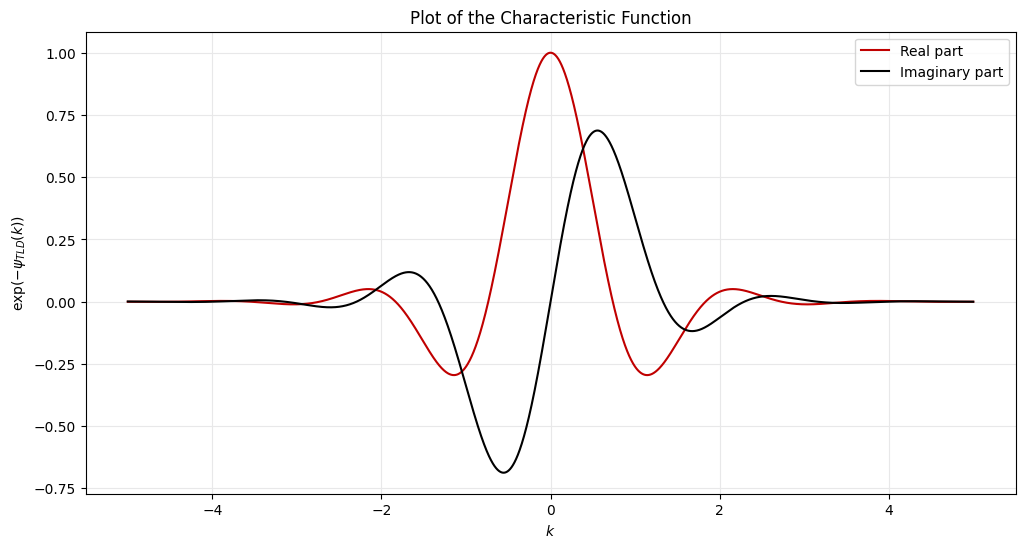
\includegraphics[width=0.6 \linewidth]{char_func}
            \caption{The characteristic function of the TSL. Parameters: $\mu=2, \,c=5,\, \alpha = 0.7, \, \lambda = 2,\, \beta =-0.8$}
            \label{fig:char_func}
        \end{figure}


        \subsection{Fitting the TSL}
        To obtain the PDF, the characteristic function (see figure~\ref{fig:char_func}) must be numerically Fourier-transformed.
        Following the paper approach, we use Romberg integration for $k \in [-15, 15]$ using $2^{12}+1$ steps.
        This calculation is computationally expensive: for a given set of the five parameters, evaluating the PDF for 1000 $x$ points takes around 5 seconds.
        As the dataset contains around 7000 observations, the calculation of the loglikelihood for a given parameter set takes around 35 seconds, or in other words,
        even a simple grid search over the parameters $\alpha, \lambda, \beta$ (as we are fitting on standardized returns, we can assume $\mu=0, c=1$) with a $7\times 7\times 7$ grid would take around 3.5 hours to complete.
        Therefore, I resorted to a faster, but less accurate approach:
        \begin{enumerate}
            \item I compute the KDE PDF of the standardized returns with bandwidth parameter given by Scott’s rule of thumb:
                    $$b = n^{-1/5}$$
            \item I evaluate the KDE PDF in a symmetric, log-spaced grid (denser around $0$) of $201$ points for $x\in [-15,15]$.
            \item I perform a grid search to find the set of parameters $\alpha, \lambda, \beta$ that minimizes the total squared error
                between the KDE PDE and the TSL PDF calculated with the given set of parameters on the points in the log-spaced grid,
                effectively reducing the number of required calls to the TSL PDF to $201$ for each parameter set.
                The grid was chosen by taking 13 equally spaced points in the following ranges:
                $$ \alpha \in [0.75,0.81], \quad \lambda \in [1.60,1.80], \quad \beta \in [-0.18,-0.12].$$
        \end{enumerate}
        In figure~\ref{fig:fitted_tls}, we see a plot of the resulting TSL PDF and in table~\ref{tab:parameters} we see the results of the grid search.\\
        Unfortunately this approach is not free of consequences in terms of accuracy, as the total mean squared error (TMSE) of the KDE PDF greatly dominates the total squared error of the grid search:
        \begin{equation}
            \begin{aligned}
                &\widehat{TMSE}_{KDE} = \frac{1}{2\sqrt{\pi}} \sum_{i=1}^{201}\widehat{\pdf}_{KDE}(x_i) = 1.88, \\
                &\widehat{TSE}_{GS} = \sum_{i=1}^{201}\bigg(\pdf_{TSL}(x_i, \hat{\alpha}, \hat{\lambda}, \hat{\beta})-\widehat{\pdf}_{KDE}(x_i)\bigg)^2 = 0.005,
            \end{aligned}
        \end{equation}
        and the errors in table~\ref{tab:parameters} are likely to severely underestimate the actual standard errors of $\hat{\alpha}, \hat{\lambda}, \hat{\beta}$ if treated as estimators of the parameters of the actual distribution of the data.

        \begin{table}[h!]
            \centering
            \begin{tabular}{c|c|c|c}
                \hline
                Parameters & $\alpha$ & $\lambda$ & $\beta$  \\
                \hline
                 Values & 0.765 & 1.67 & -0.155\\
                Absolute Errors & 0.005 & 0.01 & 0.005 \\
                Standard Errors & 0.002 & 0.006 & 0.002 \\
                \hline
            \end{tabular}
            \caption{The SE have been calculated assuming a uniform distribution in the interval where the estimate lies, and thus dividing the absolute errors by $\sqrt{3}$.
            All the errors refer to the parameter values that give origin to the KDE PDF, and not the actual distribution of the data.}
            \label{tab:parameters}
        \end{table}

        \begin{figure}[h!]
            \centering
            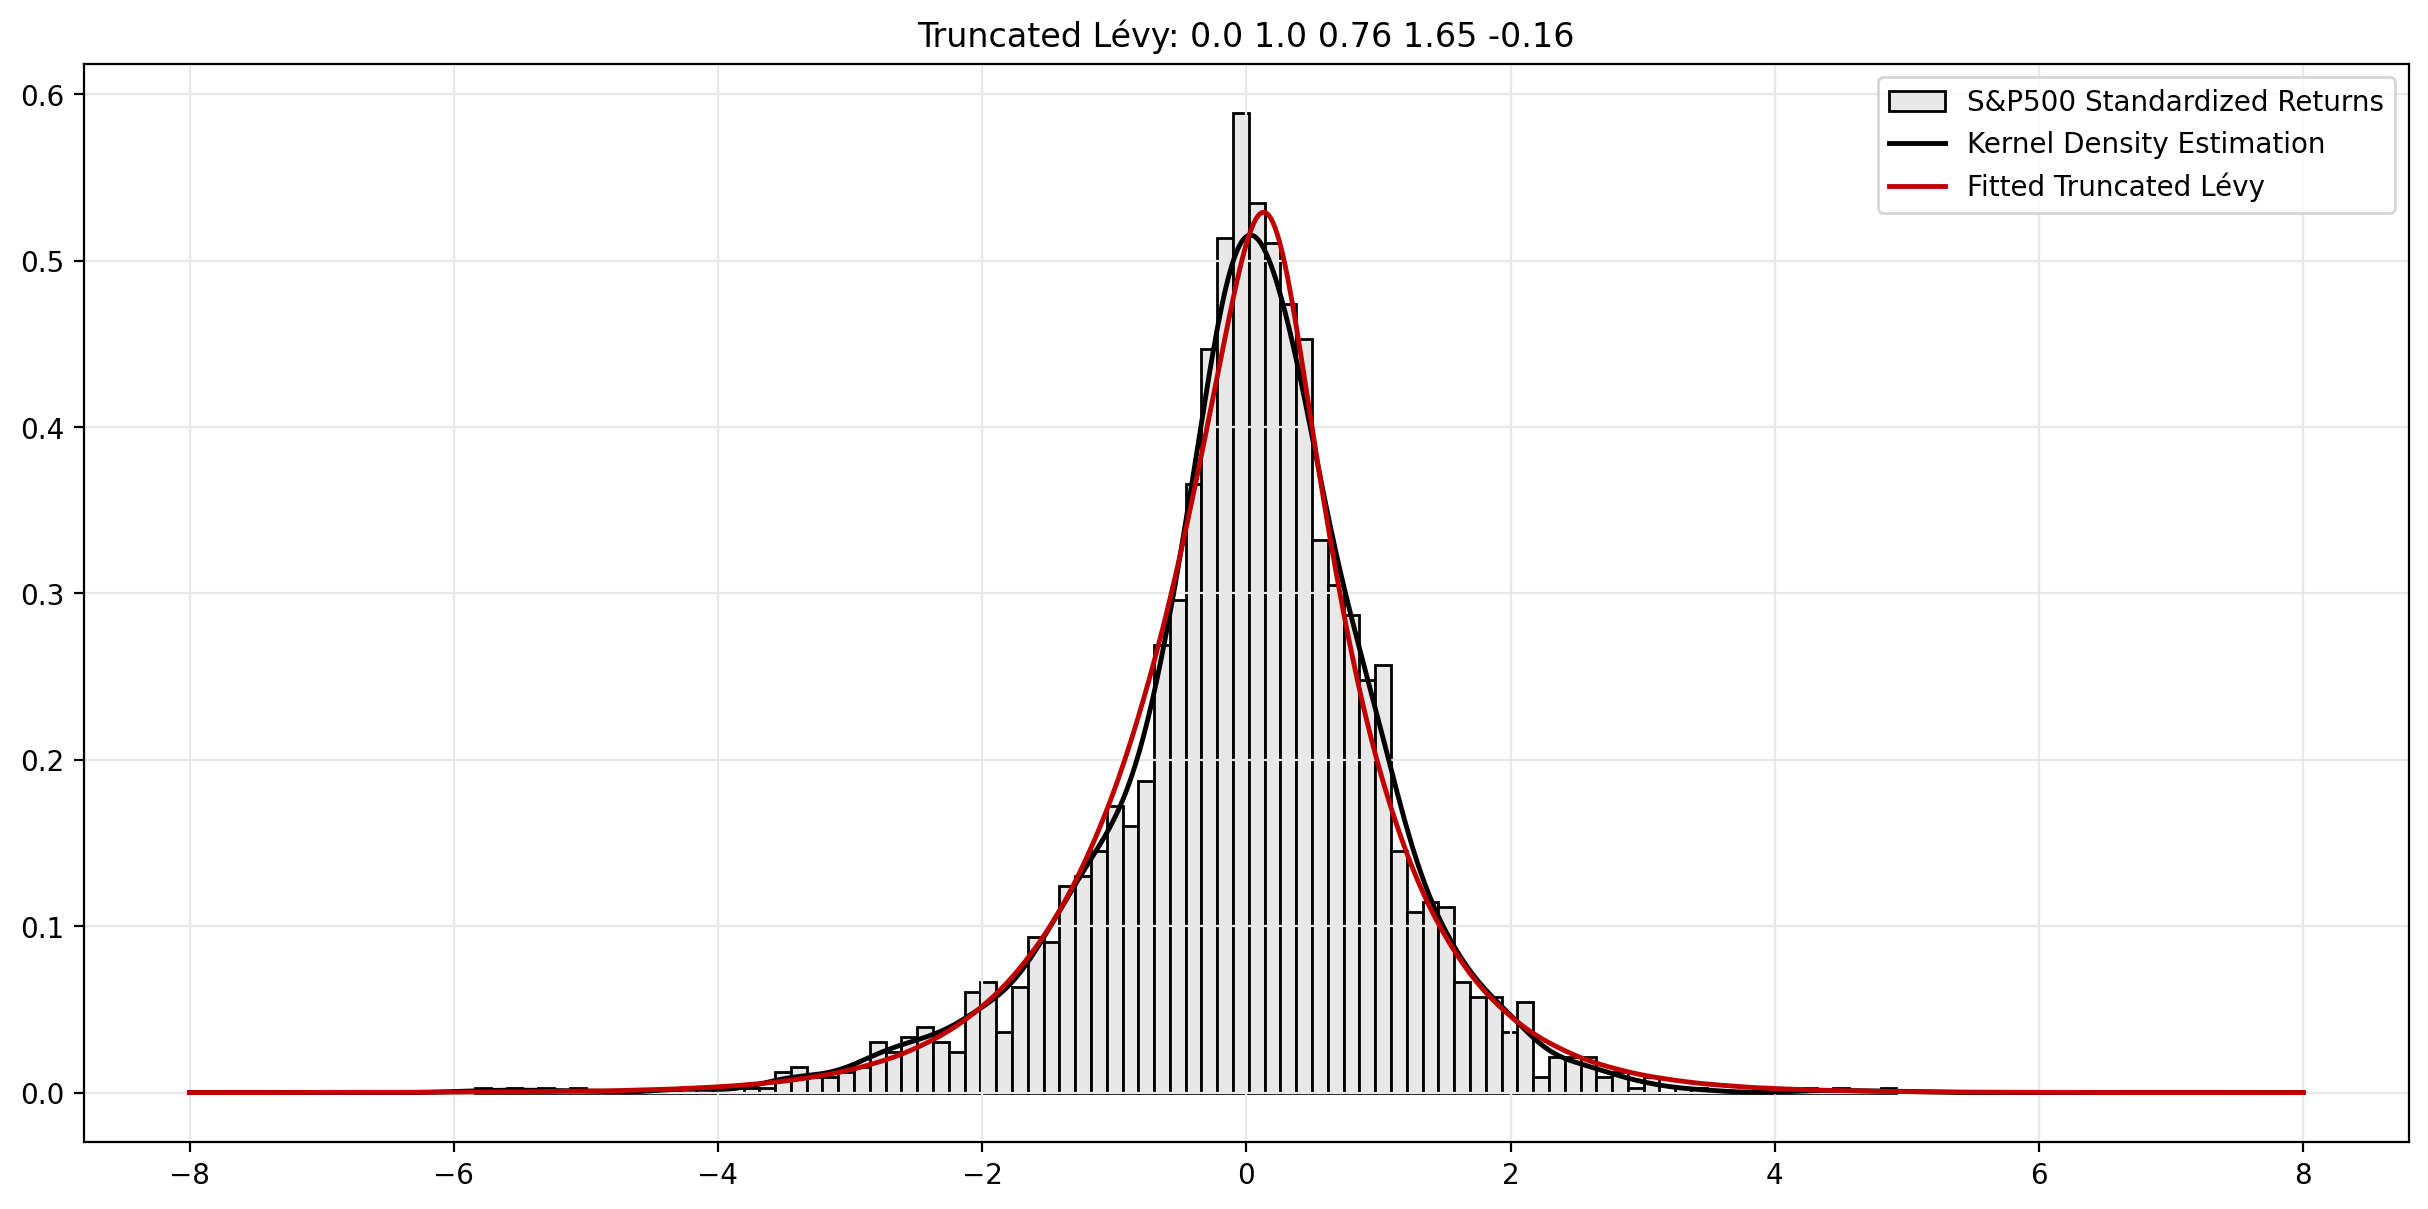
\includegraphics[width=0.6 \linewidth]{fitted_tls}
            \caption{TSL PDF obtained by calibrating the parameters over the KDE PDF, and the standardized returns.}
            \label{fig:fitted_tls}
        \end{figure}

        \subsection{Estimating the VaR}



    \section{Direct Method} \label{sec:direct}
    \subsection{Value at Risk Violations}
        On the testing set, the $\alpha$\% Value at Risk is calulated by multiplying the $\alpha$-percentile of the shock distribution with the estimated volatility (using the model calibrated on the training set).
        The estimated VaR is then compared with the actual returns, and a violation is flagged if the return is below the (negative) VaR.
\end{document}